
\documentclass[letterpaper,hide notes,xcolor={table,svgnames},pdftex,10pt]{beamer}
\def\showexamples{t}

\usecolortheme{crane}
\setbeamertemplate{navigation symbols}{}

\usetheme{MyPittsburgh}
\usepackage{hyperref}
\usepackage{graphicx,xspace}
\usepackage[normalem]{ulem}
\usepackage{multicol}
\usepackage{amsmath,amssymb,amsthm,graphicx,xspace}
\newcommand\SF[1]{$\bigstar$\footnote{SF: #1}}

\usepackage[sfdefault,lf]{carlito}
\usepackage[T1]{fontenc}
\usepackage[scaled]{beramono}
\usepackage{tikzpagenodes}
\newcommand{\Rplus}{\protect\hspace{-.1em}\protect\raisebox{.35ex}{\small{\small\textbf{+}}}}
\newcommand{\Cpp}{\mbox{C\Rplus\Rplus}\xspace}

\newcounter{tmpnumSlide}
\newcounter{tmpnumNote}

\newcommand\mnote[1]{%
	\addtocounter{tmpnumSlide}{1}
	\ifdefined\showcues {~\tiny\fbox{\arabic{tmpnumSlide}}}\fi
	\note{\setlength{\parskip}{1ex}\addtocounter{tmpnumNote}{1}\textbf{\Large \arabic{tmpnumNote}:} {#1\par}}}

\newcommand\mmnote[1]{\note{\setlength{\parskip}{1ex}#1\par}}


\newcommand\mquestion[2]{{~\color{red}\fbox{?}}\note{\setlength{\parskip}{1ex}\par{\Large \textbf{?}} #1} \note{\setlength{\parskip}{1ex}\par{\Large \textbf{A}} #2\par}\ifdefined \presentationonly \pause \fi}

\newcommand\blackboard[1]{%
	\ifdefined   \showblackboard
		{#1}
	\else {\begin{center} \fbox{\colorbox{blue!30}{%
						\begin{minipage}{.95\linewidth}%
							\hspace{\stretch{1}} Some space intentionally left blank; done at the blackboard.%
						\end{minipage}}}\end{center}}%
	\fi%
}

\usepackage{listings}
\lstset{%
	keywordstyle=\bfseries,
	aboveskip=15pt,
	belowskip=15pt,
	captionpos=b,
	identifierstyle=\ttfamily,
	frame=lines,
	numbers=left, basicstyle=\scriptsize, numberstyle=\tiny, stepnumber=0, numbersep=2pt}

\usepackage{siunitx}
\newcommand\sius[1]{\num[group-separator = {,}]{#1}\si{\micro\second}}
\newcommand\sims[1]{\num[group-separator = {,}]{#1}\si{\milli\second}}
\newcommand\sins[1]{\num[group-separator = {,}]{#1}\si{\nano\second}}
\sisetup{group-separator = {,}, group-digits = true}

%% -------------------- tikz --------------------
\usepackage{tikz}
\usetikzlibrary{positioning}
\usetikzlibrary{arrows,backgrounds,automata,decorations.shapes,decorations.pathmorphing,decorations.markings,decorations.text}

\tikzstyle{place}=[circle,draw=blue!50,fill=blue!20,thick, inner sep=0pt,minimum size=6mm]
\tikzstyle{transition}=[rectangle,draw=black!50,fill=black!20,thick, inner sep=0pt,minimum size=4mm]

\tikzstyle{block}=[rectangle,draw=black, thick, inner sep=5pt]
\tikzstyle{bullet}=[circle,draw=black, fill=black, thin, inner sep=2pt]

\tikzstyle{pre}=[<-,shorten <=1pt,>=stealth',semithick]
\tikzstyle{post}=[->,shorten >=1pt,>=stealth',semithick]
\tikzstyle{bi}=[<->,shorten >=1pt,shorten <=1pt, >=stealth',semithick]

\tikzstyle{mut}=[-,>=stealth',semithick]

\tikzstyle{treereset}=[dashed,->, shorten >=1pt,>=stealth',thin]

\usepackage{ifmtarg}
\usepackage{xifthen}
\makeatletter
% new counter to now which frame it is within the sequence
\newcounter{multiframecounter}
% initialize buffer for previously used frame title
\gdef\lastframetitle{\textit{undefined}}
% new environment for a multi-frame
\newenvironment{multiframe}[1][]{%
	\ifthenelse{\isempty{#1}}{%
		% if no frame title was set via optional parameter,
		% only increase sequence counter by 1
		\addtocounter{multiframecounter}{1}%
	}{%
		% new frame title has been provided, thus
		% reset sequence counter to 1 and buffer frame title for later use
		\setcounter{multiframecounter}{1}%
		\gdef\lastframetitle{#1}%
	}%
	% start conventional frame environment and
	% automatically set frame title followed by sequence counter
	\begin{frame}%
		\frametitle{\lastframetitle~{\normalfont(\arabic{multiframecounter})}}%
		}{%
	\end{frame}%
}
\makeatother

\makeatletter
\newdimen\tu@tmpa%
\newdimen\ydiffl%
\newdimen\xdiffl%
\newcommand\ydiff[2]{%
	\coordinate (tmpnamea) at (#1);%
	\coordinate (tmpnameb) at (#2);%
	\pgfextracty{\tu@tmpa}{\pgfpointanchor{tmpnamea}{center}}%
	\pgfextracty{\ydiffl}{\pgfpointanchor{tmpnameb}{center}}%
	\advance\ydiffl by -\tu@tmpa%
}
\newcommand\xdiff[2]{%
	\coordinate (tmpnamea) at (#1);%
	\coordinate (tmpnameb) at (#2);%
	\pgfextractx{\tu@tmpa}{\pgfpointanchor{tmpnamea}{center}}%
	\pgfextractx{\xdiffl}{\pgfpointanchor{tmpnameb}{center}}%
	\advance\xdiffl by -\tu@tmpa%
}
\makeatother
\newcommand{\copyrightbox}[3][r]{%
	\begin{tikzpicture}%
		\node[inner sep=0pt,minimum size=2em](ciimage){#2};
		\usefont{OT1}{phv}{n}{n}\fontsize{4}{4}\selectfont
		\ydiff{ciimage.south}{ciimage.north}
		\xdiff{ciimage.west}{ciimage.east}
		\ifthenelse{\equal{#1}{r}}{%
			\node[inner sep=0pt,right=1ex of ciimage.south east,anchor=north west,rotate=90]%
			{\raggedleft\color{black!50}\parbox{\the\ydiffl}{\raggedright{}#3}};%
		}{%
			\ifthenelse{\equal{#1}{l}}{%
				\node[inner sep=0pt,right=1ex of ciimage.south west,anchor=south west,rotate=90]%
				{\raggedleft\color{black!50}\parbox{\the\ydiffl}{\raggedright{}#3}};%
			}{%
				\node[inner sep=0pt,below=1ex of ciimage.south west,anchor=north west]%
				{\raggedleft\color{black!50}\parbox{\the\xdiffl}{\raggedright{}#3}};%
			}
		}
	\end{tikzpicture}
}


%% --------------------

%\usepackage[excludeor]{everyhook}
%\PushPreHook{par}{\setbox0=\lastbox\llap{MUH}}\box0}

%\vspace*{\stretch{1}

%\setbox0=\lastbox \llap{\textbullet\enskip}\box0}

\setlength{\parskip}{\fill}

\newcommand\noskips{\setlength{\parskip}{1ex}}
\newcommand\doskips{\setlength{\parskip}{\fill}}

\newcommand\xx{\par\vspace*{\stretch{1}}\par}
\newcommand\xxs{\par\vspace*{2ex}\par}
\newcommand\tuple[1]{\langle #1 \rangle}
\newcommand\code[1]{{\sf \footnotesize #1}}
\newcommand\ex[1]{\uline{Example:} \ifdefined \presentationonly \pause \fi
	\ifdefined\showexamples#1\xspace\else{\uline{\hspace*{2cm}}}\fi}

\newcommand\ceil[1]{\lceil #1 \rceil}


\AtBeginSection[]
{
	\begin{frame}
		\frametitle{Outline}
		\tableofcontents[currentsection]
	\end{frame}
}



\pgfdeclarelayer{edgelayer}
\pgfdeclarelayer{nodelayer}
\pgfsetlayers{edgelayer,nodelayer,main}

\tikzstyle{none}=[inner sep=0pt]
\tikzstyle{rn}=[circle,fill=Red,draw=Black,line width=0.8 pt]
\tikzstyle{gn}=[circle,fill=Lime,draw=Black,line width=0.8 pt]
\tikzstyle{yn}=[circle,fill=Yellow,draw=Black,line width=0.8 pt]
\tikzstyle{empty}=[circle,fill=White,draw=Black]
\tikzstyle{bw} = [rectangle, draw, fill=blue!20,
text width=4em, text centered, rounded corners, minimum height=2em]

\newcommand{\CcNote}[1]{% longname
	This work is licensed under the \textit{Creative Commons #1 3.0 License}.%
}
\newcommand{\CcImageBy}[1]{%
	\includegraphics[scale=#1]{creative_commons/cc_by_30.pdf}%
}
\newcommand{\CcImageSa}[1]{%
	\includegraphics[scale=#1]{creative_commons/cc_sa_30.pdf}%
}
\newcommand{\CcImageNc}[1]{%
	\includegraphics[scale=#1]{creative_commons/cc_nc_30.pdf}%
}
\newcommand{\CcGroupBySa}[2]{% zoom, gap
	\CcImageBy{#1}\hspace*{#2}\CcImageNc{#1}\hspace*{#2}\CcImageSa{#1}%
}
\newcommand{\CcLongnameByNcSa}{Attribution-NonCommercial-ShareAlike}

\newenvironment{changemargin}[1]{% 
	\begin{list}{}{% 
		\setlength{\topsep}{0pt}% 
		\setlength{\leftmargin}{#1}% 
		\setlength{\rightmargin}{1em}
		\setlength{\listparindent}{\parindent}% 
		\setlength{\itemindent}{\parindent}% 
		      \setlength{\parsep}{\parskip}% 
		      }% 
		\item[]}{\end{list}}




\title{Lecture 30 --- Asynchronous I/O with cURL }

\author{Jeff Zarnett \\ \small \texttt{jzarnett@uwaterloo.ca}}
\institute{Department of Electrical and Computer Engineering \\
	University of Waterloo}
\date{\today}


\begin{document}

\begin{frame}
	\titlepage

\end{frame}

\begin{frame}
	\frametitle{Using cURL}

	We've already seen that network communication is a great example of a way that you could use asynchronous I/O.

	You can start a network request and move on to creating more without waiting for the results of the first one.

	For requests to different recipients, it certainly makes sense to do this.

	And yet, we've seen that while socket programming is important and necessary, for a lot of situations we prefer to use cURL.

\end{frame}


\begin{frame}
	\frametitle{Curl Multi}

	Curl:
	\begin{center}
		
\includegraphics[width=0.2\textwidth]{images/curling.jpg}
	\end{center}

	Curl Multi:
	\begin{center}
		
\includegraphics[width=0.2\textwidth]{images/curling.jpg}
		
\includegraphics[width=0.2\textwidth]{images/curling.jpg}
		
\includegraphics[width=0.2\textwidth]{images/curling.jpg}
		
\includegraphics[width=0.2\textwidth]{images/curling.jpg}
		
\includegraphics[width=0.2\textwidth]{images/curling.jpg}
	\end{center}

	\hfill Photo Credit: J. Bourassa

\end{frame}

\begin{frame}[fragile]
	\frametitle{cURL Easy}

	Quick Recap of the Easy interface:

	\begin{lstlisting}[language=C]
#include <stdio.h>
#include <curl/curl.h>
 
int main( int argc, char** argv ) {
  CURL *curl;
  CURLcode res;
 
  curl_global_init(CURL_GLOBAL_DEFAULT);
 
  curl = curl_easy_init();
  if( curl ) {
    curl_easy_setopt(curl, CURLOPT_URL, "https://example.com/" );
    res = curl_easy_perform( curl );
    
  if( res != CURLE_OK ) {
      fprintf(stderr, "curl_easy_perform() failed: %s\n", 
      curl_easy_strerror(res));
    }
    curl_easy_cleanup(curl);
  }
 
  curl_global_cleanup();
  return 0;
}
\end{lstlisting}


\end{frame}

\begin{frame}
	\frametitle{cURL Multi}

	The call to \texttt{curl\_easy\_perform()} is blocking and we wait for the curl execution to take place.

	We want to change that!

	The tool for this is the ``multi handle'' - this is a structure that lets us have more than one curl easy handle.

	And rather than waiting, we can start them and then check on their progress.

\end{frame}


\begin{frame}
	\frametitle{Some Things Don't Change}

	There are still the global initialization and cleanup functions.

	The structure for the new multi-handle type is \texttt{CURLM}.

	It is initialized with the \texttt{curl\_multi\_init()} function.

\end{frame}


\begin{frame}
	\frametitle{Climb Aboard}

	Once we have a multi handle, we can add easy handles -- however many we need -- to the multi handle.

	Creation of the easy handle is the same as it is when being used alone - use \texttt{curl\_easy\_init()} to create it.

	Then we can set however many options on this we need.

	Then, we add the easy handle to the multi handle with \texttt{curl\_multi\_add\_handle( CURLM* cm, CURL* eh )}.


\end{frame}

\begin{frame}
	\frametitle{BOMBARDMENT!}
	\begin{center}
		
\includegraphics[width=0.7\textwidth]{images/Bombardment.png}
	\end{center}
	\hfill Image Credit: The Simpsons

	We can dispatch all easy handles at once with\\
	\texttt{curl\_multi\_perform( CURLM* cm, int* still\_running )}.


\end{frame}

\begin{frame}
	\frametitle{Still Running}

	The second parameter is a pointer to an integer that is updated with the number of the easy handles in that multi handle that are still running.

	If it's down to 0, then we know that they are all done.

	If it's nonzero it means that some of them are still in progress.


\end{frame}

\begin{frame}
	\frametitle{Asking is Okay}

	This does mean that we're going to call\texttt{curl\_multi\_perform()} more than once.

	Doing so doesn't restart or interfere with anything that was already in progress.

	We can check as often as we would like -- but we should be doing something useful rather than polling... right?

\end{frame}


\begin{frame}[fragile]
	\frametitle{Naps Are Okay}

	Suppose we've run out of things to do though. What then?

	\begin{lstlisting}[language=C]
curl_multi_wait( CURLM *multi_handle, struct curl_waitfd extra_fds[], 
    unsigned int extra_nfds, int timeout_ms, int *numfds )} . 
\end{lstlisting}

	\texttt{multi\_handle}: the multi handle to watch.

	\texttt{extra\_fds}: an array of extra file descriptors to watch (NULL).

	\texttt{extra\_nfds}: how many extra file descriptors there are (0).

	\texttt{timeout\_ms} timeout in ms... clearly...

	\texttt{numfds} updated with the number of ``interesting'' events that occurred.

\end{frame}

\begin{frame}
	\frametitle{Meanwhile...}

	In the meantime though, the perform operations are happening, and so are whatever callbacks we have set up (if any).

	And as the I/O operation moves through its life cycle, the state of the easy handle is updated appropriately.

	Each easy handle has an associated status message as well as a return code.


\end{frame}


\begin{frame}
	\frametitle{Both of them?}
	\begin{center}
		
\includegraphics[width=0.4\textwidth]{images/yoda-two.jpg}
	\end{center}

	The message could be, for example ``done'', but does that mean finished with success or finished with an error?
\end{frame}

\begin{frame}
	\frametitle{Both of them?}
	We can ask about the status of the request using \texttt{curl\_multi\_info\_read( CURLM* cm, int* msgs\_left )}.

	This returns a pointer to information ``next'' easy handle, if there is one.

	The return value is a pointer to a struct of type \texttt{CURLMsg}.

	Along side this, the parameter \texttt{msgs\_left} is updated to say how many messages remain.

\end{frame}

\begin{frame}
	\frametitle{Read Your E-mails!}

	We will therefore check the \texttt{CURLMsg} message to see what happened and make sure all is well.

	If our message that we got back with the info read is called \texttt{m}, What we are looking for is that the \texttt{m->msg} is equal to \texttt{CURLMSG\_DONE} -- request completed.

	If not, this request is still in progress and we aren't ready to evaluate whether it was successful or not.

	If done, we should look at the return code in and the result, in \texttt{m->data.result}.

	If it is \texttt{CURLE\_OK} then everything succeeded. If anything else, it indicates an error.


\end{frame}

\begin{frame}
	\frametitle{Remove Easy Handle}

	When a handle has finished, you need to remove it from the multi handle.

	A pointer to it is inside the \texttt{CURLMsg} under \texttt{m->easy\_handle}.

	It is removed with \texttt{curl\_multi\_remove\_handle( CURLM* cm, CURL eh )}.

	Once removed, clean it up with: \texttt{curl\_easy\_cleanup( CURL* eh )}.


\end{frame}

\begin{frame}
	\frametitle{Clean the Multi}

	There is the multi cleanup function \texttt{curl\_multi\_cleanup( CURLM * cm ) }.

	The last step, as before, is to use the global cleanup function.

	After that we are done.


\end{frame}

\begin{frame}[fragile]
	\frametitle{cURL Multi Example}

	\begin{lstlisting}[language=C]
#include <stdio.h>
#include <stdlib.h>
#include <unistd.h>
#include <curl/multi.h>

#define MAX_WAIT_MSECS 30*1000 /* Wait max. 30 seconds */

const char *urls[] = {
  "http://www.microsoft.com",
  "http://www.yahoo.com",
  "http://www.wikipedia.org",
  "http://slashdot.org"
};
#define CNT 4

size_t cb(char *d, size_t n, size_t l, void *p) {
  /* take care of the data here, ignored in this example */
  return n*l;
\end{lstlisting}

\end{frame}

\begin{frame}[fragile]
	\frametitle{cURL Multi Example}

	\begin{lstlisting}[language=C]
void init( CURLM *cm, int i ) {
  CURL *eh = curl_easy_init();
  curl_easy_setopt( eh, CURLOPT_WRITEFUNCTION, cb );
  curl_easy_setopt( eh, CURLOPT_HEADER, 0L );
  curl_easy_setopt( eh, CURLOPT_URL, urls[i] );
  curl_easy_setopt( eh, CURLOPT_PRIVATE, urls[i]) ;
  curl_easy_setopt( eh, CURLOPT_VERBOSE, 0L );
  curl_multi_add_handle( cm, eh );
}

int main( int argc, char** argv ) {
    CURLM *cm = NULL;
    CURL *eh = NULL;
    CURLMsg *msg = NULL;
    CURLcode return_code = 0;
    int still_running = 0; 
    int msgs_left = 0;
    int http_status_code;
    const char *szUrl;

    curl_global_init( CURL_GLOBAL_ALL );
    cm = curl_multi_init( );
    
    for ( int i = 0; i < CNT; ++i ) {
        init( cm, i );
    }
\end{lstlisting}

\end{frame}

\begin{frame}[fragile]
	\frametitle{cURL Multi Example}

	\begin{lstlisting}[language=C]
    curl_multi_perform( cm, &still_running );

    do {
        int numfds = 0;
        int res = curl_multi_wait( cm, NULL, 0, MAX_WAIT_MSECS, &numfds );
        if( res != CURLM_OK ) {
            fprintf( stderr, "error: curl_multi_wait() returned %d\n", res );
            return EXIT_FAILURE;
        }
        curl_multi_perform( cm, &still_running );

    } while( still_running );
\end{lstlisting}

\end{frame}

\begin{frame}[fragile]
	\frametitle{cURL Multi Example}

	\begin{lstlisting}[language=C]
    while ( ( msg = curl_multi_info_read( cm, &msgs_left ) ) ) {
        if ( msg->msg == CURLMSG_DONE ) {
            eh = msg->easy_handle;
            return_code = msg->data.result;
            if ( return_code != CURLE_OK ) {
                fprintf( stderr, "CURL error code: %d\n", msg->data.result );
                continue;
            }

            http_status_code = 0;
            szUrl = NULL;
            curl_easy_getinfo( eh, CURLINFO_RESPONSE_CODE, &http_status_code );
            curl_easy_getinfo( eh, CURLINFO_PRIVATE, &szUrl );

            if( http_status_code == 200 ) {
                printf( "200 OK for %s\n", szUrl ) ;
            } else {
                fprintf( stderr, "GET of %s returned http status code %d\n",
                     szUrl, http_status_code );
            }
            curl_multi_remove_handle( cm, eh );
            curl_easy_cleanup( eh );
        } else {
            fprintf( stderr, "error: after curl_multi_info_read(), CURLMsg=%d\n",
                 msg->msg );
        }
    }

}
\end{lstlisting}

\end{frame}

\begin{frame}[fragile]
	\frametitle{cURL Multi Example}

	\begin{lstlisting}[language=C]
    curl_multi_cleanup( cm );
    curl_global_cleanup();
    return 0;
}
\end{lstlisting}

\end{frame}

\begin{frame}
	\frametitle{Recycle, Reduce, Reuse}

	\begin{center}
		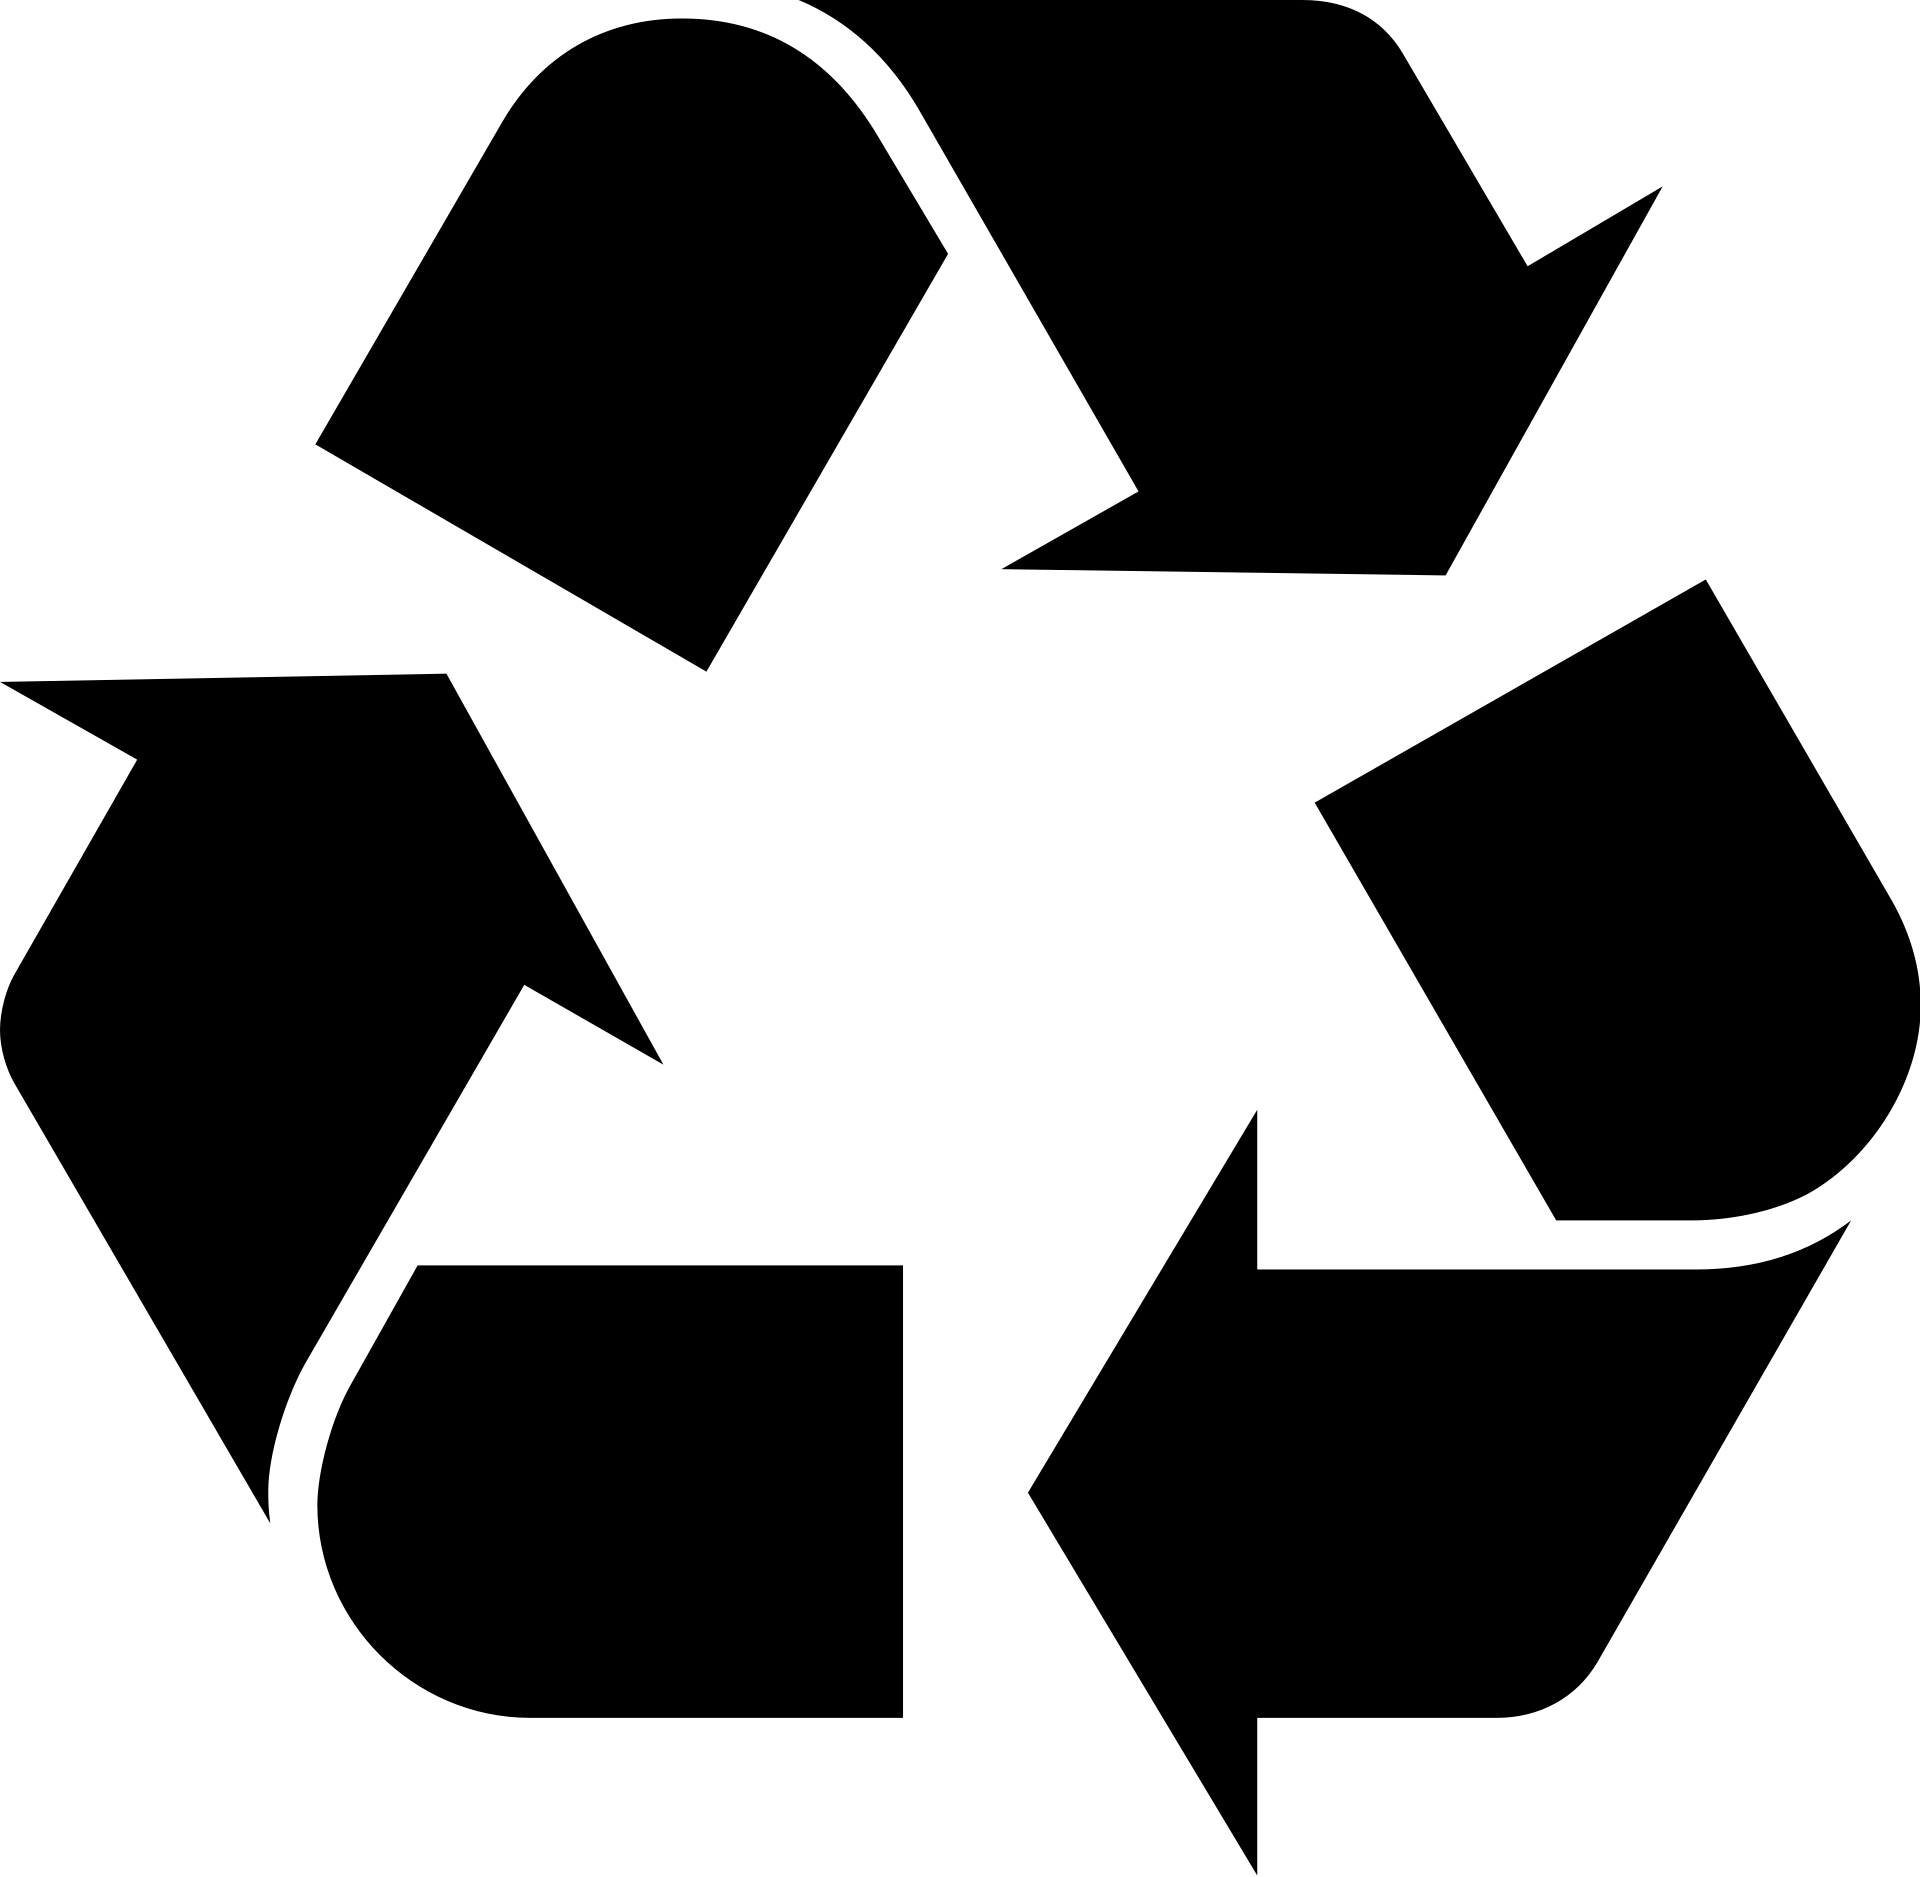
\includegraphics[width=0.3\textwidth]{images/recycle.png}
	\end{center}
	\hfill Image Credit: Wikipedia user Krdan

	Can we re-use an easy handle rather than destroy and create a new one?

\end{frame}

\begin{frame}
	\frametitle{Recycle, Reduce, Reuse}

	The official docs say that you can re-use one.

	But you have to remove it from the multi handle and then re-add it.

	... presumably after having changed anything that you want to change about that handle.

\end{frame}


\begin{frame}
	\frametitle{Always Running}

	You could have a situation where there are constantly handles in progress.

	You might never be at a situation where there are no messages left.

	And that is okay.

\end{frame}

\begin{frame}
	\frametitle{Scaling This}

	The developer claims that you can have multiple thousands of connections in a single multi handle.

	60k ought to be enough for anyone!
\end{frame}


\begin{frame}
	\frametitle{cURL + select}
	\begin{center}
		
\includegraphics[width=0.55\textwidth]{images/harold.jpg}
	\end{center}


\end{frame}


\begin{frame}[fragile]
	\frametitle{cURL + select}

	Well, alright, if you insist...

	The first part of using cURL with select is of course setting up your multi handle and adding all of the easy handles to that.

	Once you've done that, you can ask cURL to prep things for you:

	\begin{lstlisting}[language=C]
CURLMcode curl_multi_fdset( CURLM *multi_handle, fd_set *read_fd_set,
    fd_set *write_fd_set, fd_set *exc_fd_set, int *max_fd );
\end{lstlisting}

	It takes as arguments, the multi handle, and then pointers to the \texttt{fd\_set}s.

	It's the responsibility of the caller to set these to zero with \texttt{FD\_ZERO} first.

	The function is kind enough to tell you what the maximum file descriptor is.

\end{frame}

\begin{frame}[fragile]
	\frametitle{cURL + select}

	\begin{lstlisting}[language=C]
fd_set fdr;
fd_set fdw;
fd_set fde;
FD_ZERO( &fdr );
FD_ZERO( &fdw );
FD_ZERO( &fde );
int maxfd = -1;

CURLMCode res = curl_multi_fdset( cm, &fdr, &fdw, &fde, &maxfd );
\end{lstlisting}

	When calling select we still have to put a \texttt{+1} on the max file descriptor, but that is no big deal.

	The missing element is the timeout. For that there is another function:

	\begin{lstlisting}[language=C]
CURLMcode curl_multi_timeout( CURLM *multi_handle, long *timeout );
\end{lstlisting}

	Unfortunately, though, this returns a \texttt{long}...

\end{frame}


\begin{frame}[fragile]
	\frametitle{Guys, Why Can't You Get Along...}

	So you have to do the math yourself.

	Use this!

	\begin{lstlisting}[language=C]
struct timeval timeout;
long timeo;
 
curl_multi_timeout( cm, &timeo );
if(timeo < 0) {
  /* no set timeout, use a default */
  timeo = 980;
}
 
timeout.tv_sec = timeo / 1000;
timeout.tv_usec = (timeo % 1000) * 1000;
\end{lstlisting}

\end{frame}


\begin{frame}
	\frametitle{Are We Forgetting Something?}

	But we aren't ready to call \texttt{select} yet -- we haven't started any of the transfers  that use the sockets.

	For that we use \texttt{curl\_multi\_perform} just as in the earlier example.

	We can do that before or after setting up what we need for select.

\end{frame}


\begin{frame}
	\frametitle{Waking Up From a Nap}

	When we wake up, it is because something happened.

	We still use \texttt{curl\_multi\_info\_read} to find out what's going on with a given easy handle and find out its status and also find out how many are still running.

	As with the earlier code where we used \texttt{select} on sockets directly, we have to remember to reset (repopulate) the values.

\end{frame}


\begin{frame}
	\frametitle{Select Headaches}

	One of the other problems with \texttt{select} is that you are limited in the number of file descriptors because you could overflow the bitmasks.

	But even if you don't, this really does not scale, so you would be better off using the regular curl multi call.

	As far as I can see it's better in pretty much every way.

\end{frame}

\begin{frame}
	\frametitle{Poll? Nope}

	Can we use cURL with \texttt{poll}? Generally, no.

	Long story short: don't.

\end{frame}




\end{document}

